\section*{Exercícios do Bishop}

\begin{enumerate}[label=E\arabic*]

%%%%%%%%%%%%%%%%%%%%%%%%%%%%%%%%%%%%%%%%%%%%%%%%%%%%%%%%%%%%%%%

\item \textbf{Inferência Bayesiana sequencial} \par
Motivado pela Figura 2.3 do livro, reproduza o
experimento da jogada de moeda considerando que foram realizadas 5 jogadas e que a
probabilidade de se obter cara é dada por `$\mu = 0,7$'. Plote a distribuição a priori e todas
as 5 distribuições a posteriori geradas ao longo do processo iterativo. Considere que a
distribuição a priori é uma Beta com parâmetros `$a$' e `$b$' escolhidos da seguinte forma:

1º caso: $a = b = 1$

2º caso: $a = b = 2$

Compare os resultados obtidos nos 2 casos.

OBS: Para uma comparação justa entre os 2 casos, primeiro gere os 5 dados (saídas do
experimento da moeda, amostrados da Bernoulli definida no enunciado) e depois aplique
o aprendizado sequencial para os 2 casos (i.e., para ambas as prioris) usando
exatamente os mesmos dados gerados.
\begin{figure}[H]
    \caption*{\textbf{Figura 2.3 do Bishop}}
       \centering
       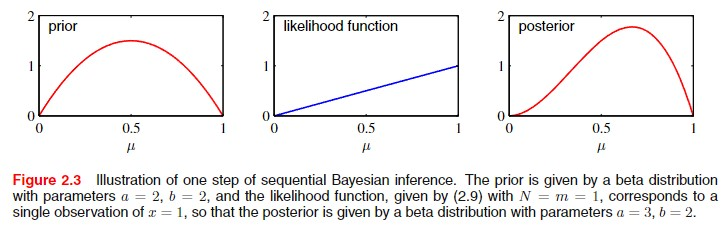
\includegraphics{bishop_23.jpg}
\end{figure}
\par
\textbf{Solução:}


%%%%%%%%%%%%%%%%%%%%%%%%%%%%%%%%%%%%%%%%%%%%%%%%%%%%%%%%%%%%%%%


\item \textbf{Verificação experimental do Teorema Central do Limite} \par
Considere a média de N variáveis aleatórias iid. Plote o histograma dessa média considerando que as N variáveis aleatórias têm a seguinte pdf:

1o caso: Uniforme(0,1) - uniforme no intervalo 0 a 1;

2o caso: Bernoulli - escolha o valor do parâmetro como quiser;

Note que, para N suficientemente grande, a distribuição da média converge para uma Gaussiana.

OBS: Usei média ao invés de soma para facilitar a geração do histograma (o eixo horizontal vai ficar fixo, facilitando a comparação para diferentes valores de N, igual na Figura 2.6 do livro).

\begin{figure}[H]
    \caption*{\textbf{Figura 2.6 do Bishop}}
       \centering
       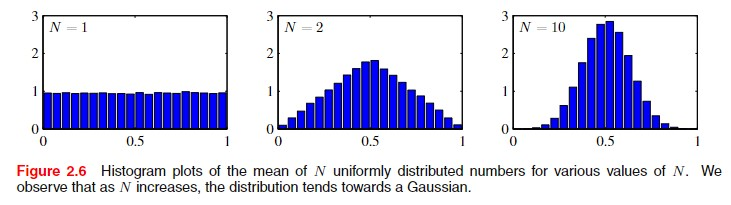
\includegraphics{bishop_26.jpg}
\end{figure}
\par
\textbf{Solução:}


%%%%%%%%%%%%%%%%%%%%%%%%%%%%%%%%%%%%%%%%%%%%%%%%%%%%%%%%%%%%%%%

\item \textbf{Verificação experimental da Law of Large Numbers - LLN} \par
Considere N variáveis aleatórias independentes geradas a partir de uma distribuição normal padrão (isto é, Gaussiana de média 0 e variância 1). Compute o estimador média amostral. Repita o experimento diversas vezes e plote o histograma desse estimador para um dado valor de N. Mostre que, conforme N aumenta, o histograma desse estimador fica cada vez mais estreito em torno do valor correto (i.e., variância vai diminuindo), que é zero.
\par
\textbf{Solução:}


%%%%%%%%%%%%%%%%%%%%%%%%%%%%%%%%%%%%%%%%%%%%%%%%%%%%%%%%%%%%%%%

\item \textbf{Estimação de pdf} \par
Tente replicar os resultados exibidos nas figuras 2.24 e 2.25 do livro. Para isso, gere uma amostra de N=50 dados cuja distribuição é dada pela curva em verde (corresponde a uma mistura de 2 gaussianas - veja equação 
$$p(x) = \sum_{k=1}^{K}\pi_k \mathcal{N} (x|\mu_k. \Sigma_k)$$ 
e escolha os parâmetros dessa distribuição da forma que quiser). Estime a pdf do modelo gerador dos dados utilizando 2 métodos: histograma e kernel Gaussiano. Para o parâmetro h, utilize os mesmos valores das figuras.
\begin{figure}[H]
    \caption*{\textbf{Figura 2.24 do Bishop}}
       \centering
       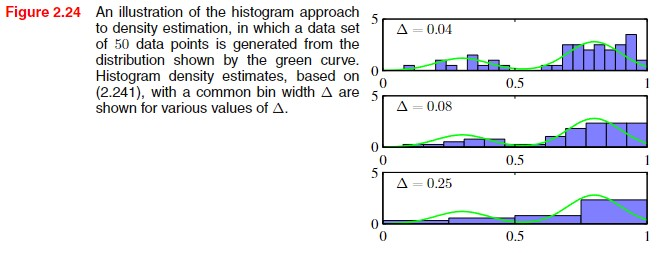
\includegraphics{bishop_224.jpg}
\end{figure}
\begin{figure}[H]
    \caption*{\textbf{Figura 2.25 do Bishop}}
       \centering
       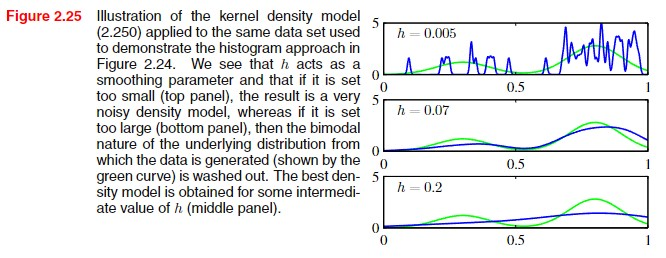
\includegraphics{bishop_225.jpg}
\end{figure}
\par
\textbf{Solução:}


%%%%%%%%%%%%%%%%%%%%%%%%%%%%%%%%%%%%%%%%%%%%%%%%%%%%%%%%%%%%%%%

\item \textbf{Classificador K-NN} \par
Considere 2 classes, C1 e C2, que correspondem aos seguintes modelos geradores: 

C1: pdf Gaussiana de média -1 e variância 1

C2: pdf Gaussiana de média 1 e variância 1

Gere 10 observações de cada uma dessas classes e assuma que você sabe exatamente a classe de cada um dos 20 pontos gerados (10 pontos para cada classe). Em seguida, gere mais 2 observações de cada classe e assuma que você NÃO sabe de qual classe esses novos dados pertencem. Utilize a técnica de K-NN, considerando diferentes valores de K, para classificar os 4 novos dados.

OBS: Plote os resultados utilizando cores e símbolos para facilitar a interpretação. Por exemplo: Para os 20 pontos conhecidos, represente-os usando `bolinhas' vermelhas para C1 e azuis para C2. Para os 4 pontos a serem classificados, mantenha o código de cores (para sabermos identificar qual era a classe correta) e use novos símbolos para identificar se a classificação foi correta (use um `quadrado') ou se a classificação foi errada (neste caso, use um `x').

Se for usar outros símbolos e cores, não tem problema. Só não esqueça de fazer uma
legenda ou caption que me permita compreender a figura.


\par
\textbf{Solução:}


%%%%%%%%%%%%%%%%%%%%%%%%%%%%%%%%%%%%%%%%%%%%%%%%%%%%%%%%%%%%%%%



\end{enumerate}